\subsection{Feature extraction} \label{subsec:feature-extraction}

Audio data comes in the shape of vectors of audio samples, one per microphone
channel. These vectors contain the audio amplitude for a single time instant.
The time between consecutive audio samples is defined by the sampling frequency
(or sample rate) of the audio recording.

However individual audio samples are not very informative, the key information
lies behind the oscillation of consecutive samples. That's why it is a very
common practice to represent audio features in the frequency domain.

The term \emph{extractor} will be used to abstract the system used to extract
features from audio data. Although in this work only one type of extractor has
been implemented and tested, the system is designed to be generic. Additional
feature extractors, like the traditional Mel-frequency Cepstrum Coefficients
(MFCC) or a simple Short-Time Fourier Transform, can be easily implemented as
an \emph{extractor}. This work opts to use a feature extractor based on
\nameref{para:gammatone-filterbank} since the performance of
classification systems relying on MFCCs is greatly reduced in the presence of
noise \cite{marchegiani2018a}.

\paragraph{Gammatone filterbanks} \label{para:gammatone-filterbank}

An approximation to the human cochlear frequency selectivity originally
introduced in \cite{GTF1998}. Time-independent features are obtained by
filtering the audio waveform with a bank of gammatone band-pass filters. The
impulse response of a gammatone filter centered at frequency $f_c$ is given by
\cref{eq:gammatone-filter-impulse}, where $n$ indicates the order of the filter
which largely determines the slope of the filter's skirts; and $b$ is the
bandwidth of the filter and largely determines the duration of the impulse
response; $a$ is the amplitude and $\phi$ is the phase.

\begin{equation}
    g(t, f_c) = a t^{n-1}e^{-2 \pi b t} \cos{2 \pi f_c t + \phi}
    \label{eq:gammatone-filter-impulse}
\end{equation}

This work implements a bank of fourth order gammatone filters with its
corresponding bandwidth $b$ of 1.019 ERB where ERB is the equivalent
rectangular bandwidth scale \cite{GLASBERG1990103}. Said implementation is
written in C++ as a Python extension module. It is based on a Matlab MEX
function implemented in C by \citeauthor{CorrelogramMa2007}
\cite{CorrelogramMa2007}, which at the same time is based on
\citeauthor{Cooke1993ModellingAP}'s Ph.D work \cite{Cooke1993ModellingAP}. The
filters are distributed over a predefined frequency range linearly on the ERB
scale. The number of filters used is equivalent to the number of features to be
extracted. 

\subsubsection{Segmenting} \label{subsec:segments}

\Cref{sec:experimental-setup} described how 168 recordings were gathered from
the \nameref{para:single-wheel-testbed} with different driving
conditions. These recordings vary in length but they are all in the order of
magnitude of tenths of seconds. However, an odometry estimation model should be
able to make new predictions several times per second. Therefore the model
should be fed new data several times per second as well. 

The term \emph{frame} is defined as the group of vectors of features extracted
from a finite number of samples. One vector per \emph{extractor} (as defined in
\cref{subsec:feature-extraction}) used. \Cref{fig:datasets-frames} illustrates
how an audio signal is divided into frames. The number of samples per frame can
be tied together with the sample rate of the audio signal to define frames in
terms of time. Frame duration is one of the parameters of the dataset as well
as the number of features extracted per frame. \Cref{table:datasets-parameters}
lists all the different parameters that define a dataset.

\begin{figure}
    \centering
    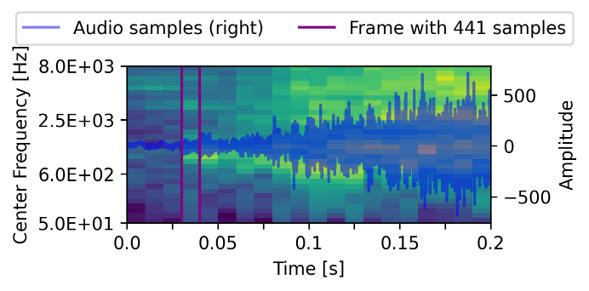
\includegraphics[width=\textwidth]{\subdir/frames.png}
    \caption[Audio frames]{Audio signal (in {\color{blue} blue}) over its
        features extracted from frames with a duration of 10 ms with a single
        \nameref{para:gammatone-filterbank} extractor.}
    \label{fig:datasets-frames}
\end{figure}

The term \emph{segment} is defined as a group of consecutive frames. Segments
will be the input for prediction models. Segments can be overlapped in a way
that consecutive segments share a percentage of their frames.
\Cref{fig:datasets-segments} how the audio frames are grouped into segments
that overlap each other.

\subsubsection{Labeling} \label{subsec:labeling}

\emph{Dataset} is defined in the context of this work as a collection of
segments annotated with their corresponding ground truth. The variables of
interest are the longitudinal velocity $V_x$, the wheel angular speed
$V_\omega$ and the slip ratio $s$. However, as it has been explained in
\cref{subsec:segments}, these segments are relatively large in terms of time.
In a way that the measured variables can oscillate significantly during the
segment. This work annotates the segments with a weighted average of the
measurements within its duration. Consider $x[t]$ the measurement of a given
variable $x$ at time $t$, being $t$ in the set of measurement times $t \in T$.
\Cref{eq:segment-labeling} describes how the weighted average of that variable
$x$ is computed for segment $k$ where $t_k$ is the vector of measurement times
inside the segment boundaries and $N$ its size.

\begin{equation}
    x_k = \frac{\sum_{i = 1}^N i  x[t_k[i]]}{\sum_{i = 1}^N i}\text{, where } i \in  \mathbb{N}
    \label{eq:segment-labeling}
\end{equation}

One can visualize in \cref{fig:datasets-segments} the segments with their
longitudinal velocity $V_x$ annotations computed from the measurements that lay
inside the segment boundaries as described by \cref{eq:segment-labeling}.
Moreover, \cref{fig:dataset-visualization} shows consecutive segments from one
of the datasets used in this work with their complete annotations.
\Cref{fig:dataset-visualization} also shows the distribution of the values of
the variables of interest in the dataset. This distribution can be altered
employing \nameref{subsec:data-augmentation} and \nameref{subsec:data-split} in
order to obtain a more favorable distribution for model training.

\begin{figure}
    \centering
    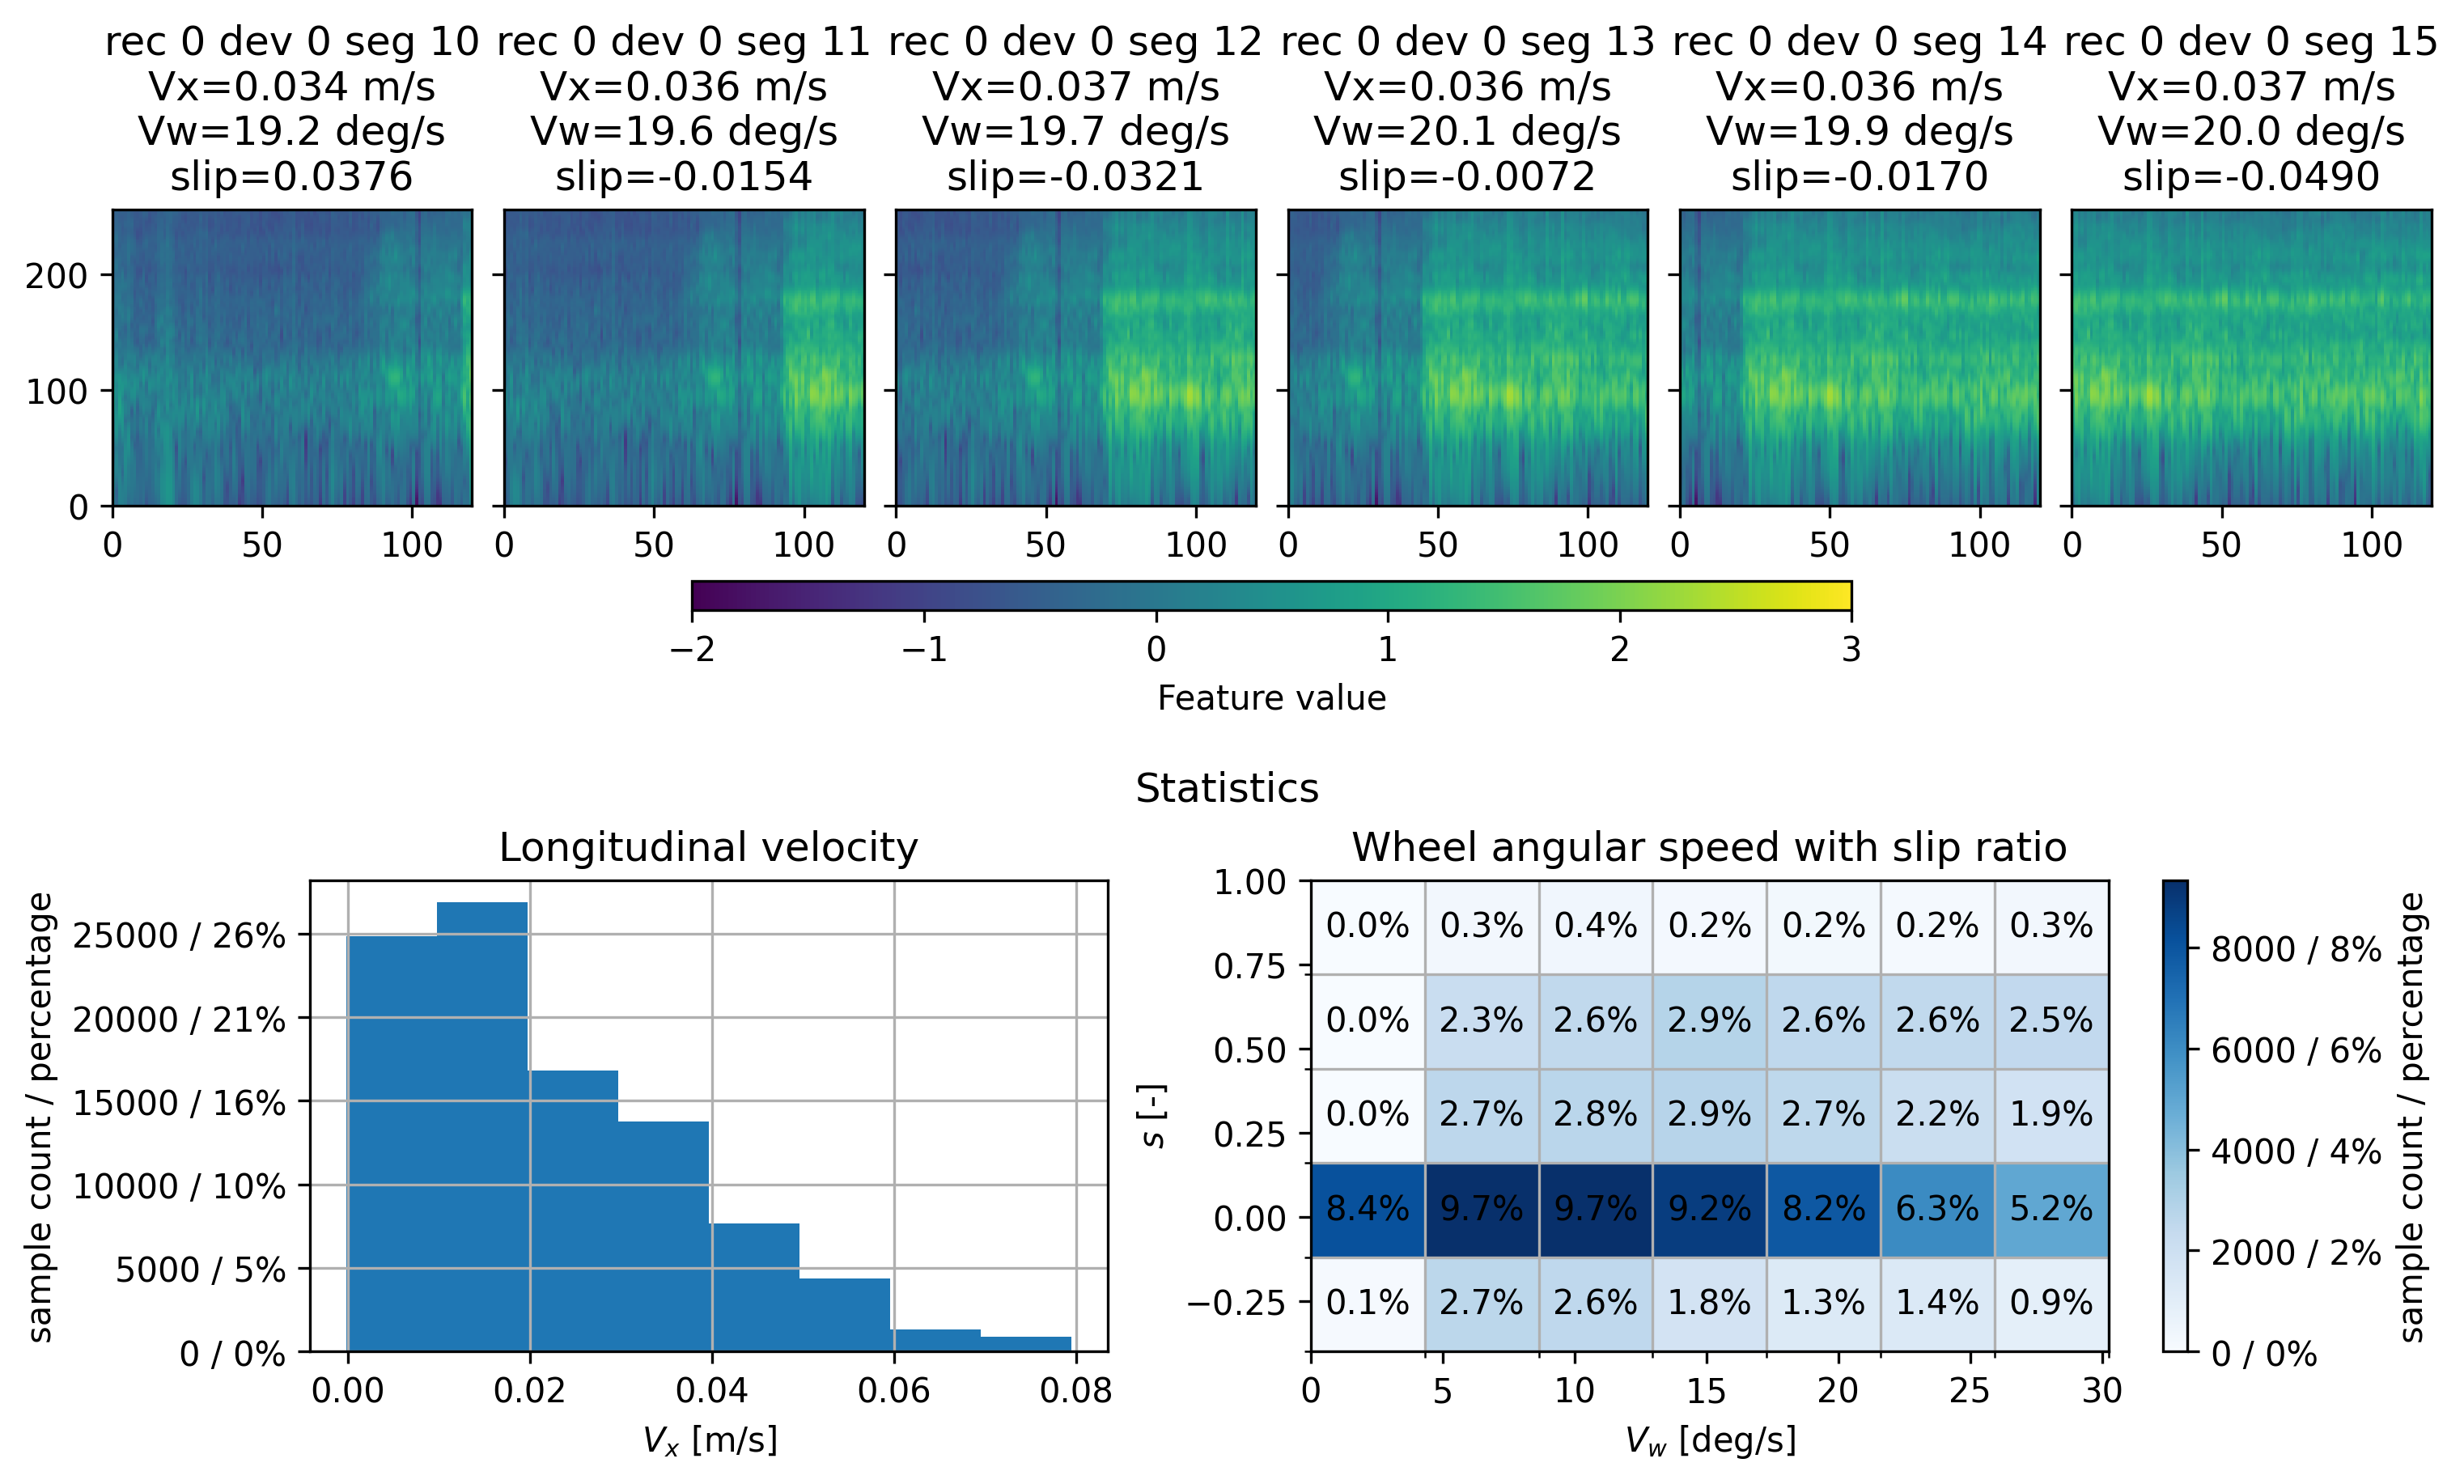
\includegraphics[width=\linewidth]{\subdir/dataset.png}
    \caption[Dataset visualization]{Visualization of consecutive samples from a
        dataset together with the distribution of the variables of interest.
        This dataset was processed using all available recordings from
        \nameref{subsec:wheel-testbed-experiment-2}, a single
        \nameref{para:gammatone-filterbank} extractor with 256 features
        per frame, a frame duration of 10 ms and a segment length of 100 frames
        with 80\% overlapped frames between consecutive segments. }
    \label{fig:dataset-visualization}
\end{figure}

\subsubsection{Data augmentation} \label{subsec:data-augmentation}

The performance of most Machine Learning models depends on the quality,
quantity, and relevancy of the training data. Artificially augmenting the data
in a dataset can be useful to improve the performance of a model. In this work
datasets are augmented by altering the raw recordings before the
\nameref{subsec:feature-extraction} and \nameref{subsec:segments} operations.
The term \emph{transform} is defined as the function to be applied to the raw
recording. Two transform functions for data augmentation are used in this work:

\begin{itemize}
    \item Gain: Add a random gain in the range [-10, 10]. Illustrated by the
          second row of samples in \cref{fig:augmented-samples}.
    \item Noise: Add white noise with a random signal-to-noise ratio in the
          range [0, 1] in the decibel scale. Illustrated by the third row of
          samples in \cref{fig:augmented-samples}.
\end{itemize}

\Cref{fig:augmented-samples} illustrates the effect of the data augmentation on
the dataset segments. The size of the dataset is essentially multiplied by the
number of transformations applied. While this improves the training data
quantity, it may decrease its quality. \Cref{subsec:data-split} describes
the techniques used to split the dataset, controlling the quality of the
training data.